\documentclass[11pt,a4paper]{article}

% ----------------------------------------------------------------------
% Project BEACON — Corporate Finance report (Kartik Joshi)
% Compile with pdfLaTeX on Overleaf. Upload the 7 PNGs from the
% screenshots/ folder into the project (same folder as this file, or a
% subfolder named "screenshots").
% ----------------------------------------------------------------------
\usepackage[margin=2.5cm]{geometry}
\usepackage{amsmath,amssymb}
\usepackage{graphicx}
\usepackage{booktabs}
\usepackage{array}
\usepackage{xcolor}
\usepackage{caption}
\usepackage{enumitem}
\usepackage{float}
\usepackage{tikz}
\usepackage{eso-pic}
\usepackage[hidelinks]{hyperref}

\graphicspath{{./}{./screenshots/}{../screenshots/}}
\captionsetup{font=small,labelfont=bf}
\renewcommand{\arraystretch}{1.25}
\setlength{\parskip}{0.5em}
\setlength{\parindent}{0pt}

% --- Single-line black border on every page ---
\AddToShipoutPictureBG{%
  \begin{tikzpicture}[remember picture,overlay]
    \draw[line width=0.6pt]
      ([shift={(1cm,1cm)}]current page.south west)
      rectangle
      ([shift={(-1cm,-1cm)}]current page.north east);
  \end{tikzpicture}%
}

\newcommand{\aed}{AED\,}

\begin{document}

% ======================================================================
% TITLE PAGE
% ======================================================================
\begin{titlepage}
\centering
\vspace*{1.2cm}

{\large\scshape Corporate Finance}\\[0.4cm]
{\rule{0.55\textwidth}{0.4pt}}\\[1.0cm]

{\Huge\bfseries Project BEACON}\\[0.6cm]
{\Large\itshape Where should Cardamom \& Co.\\open its next branch --- and is it worth opening?}\\[1.2cm]

{\rule{0.55\textwidth}{0.4pt}}\\[1.0cm]

{\normalsize Submitted for the partial fulfilment of the requirements of the\\
Corporate Finance module of the Masters in Artificial Intelligence with Business.}\\[1.6cm]

\begin{tabular}{@{}r@{\hskip 0.6cm}l@{}}
\textbf{Subject} & Corporate Finance\\[0.35cm]
\textbf{Instructor} & [Instructor Name]\\[0.35cm]
\textbf{Student} & Kartik Joshi\\[0.35cm]
\textbf{Working application} & \href{https://beacon-intelligence.vercel.app/}{beacon-intelligence.vercel.app}\\
\end{tabular}

\vfill
{\rule{\textwidth}{0.4pt}}\\[0.3cm]
{\small\itshape Topic --- Capital Budgeting: a multi-metric appraisal of a mutually-exclusive new-branch investment decision.}\\[0.3cm]
{\rule{\textwidth}{0.4pt}}
\end{titlepage}

% ======================================================================
% TABLE OF CONTENTS
% ======================================================================
\tableofcontents
\thispagestyle{plain}
\newpage

% ======================================================================
% BODY
% ======================================================================
\section{Company and Project Background}
Cardamom \& Co.\ is a Dubai-based specialty-coffee and bakehouse chain (a realistic fictional company) that runs several profitable outlets across the emirate. Buoyed by strong same-store sales, management intends to expand by opening \emph{one} additional branch in the coming financial year. Three sites have been short-listed: a flagship kiosk-caf\'e in The Dubai Mall (Site~A), a high-street unit in Jumeirah Lakes Towers (Site~B), and a delivery-only ``cloud kitchen'' (Site~C). Because the capital budget funds only one opening, the sites are \textbf{mutually exclusive}. The appraisal is carried out with the accompanying web application, \emph{Project BEACON}, which computes every capital-budgeting measure client-side and layers an AI advisor over the results (Figure~\ref{fig:overview}).

\begin{figure}[h]
\centering
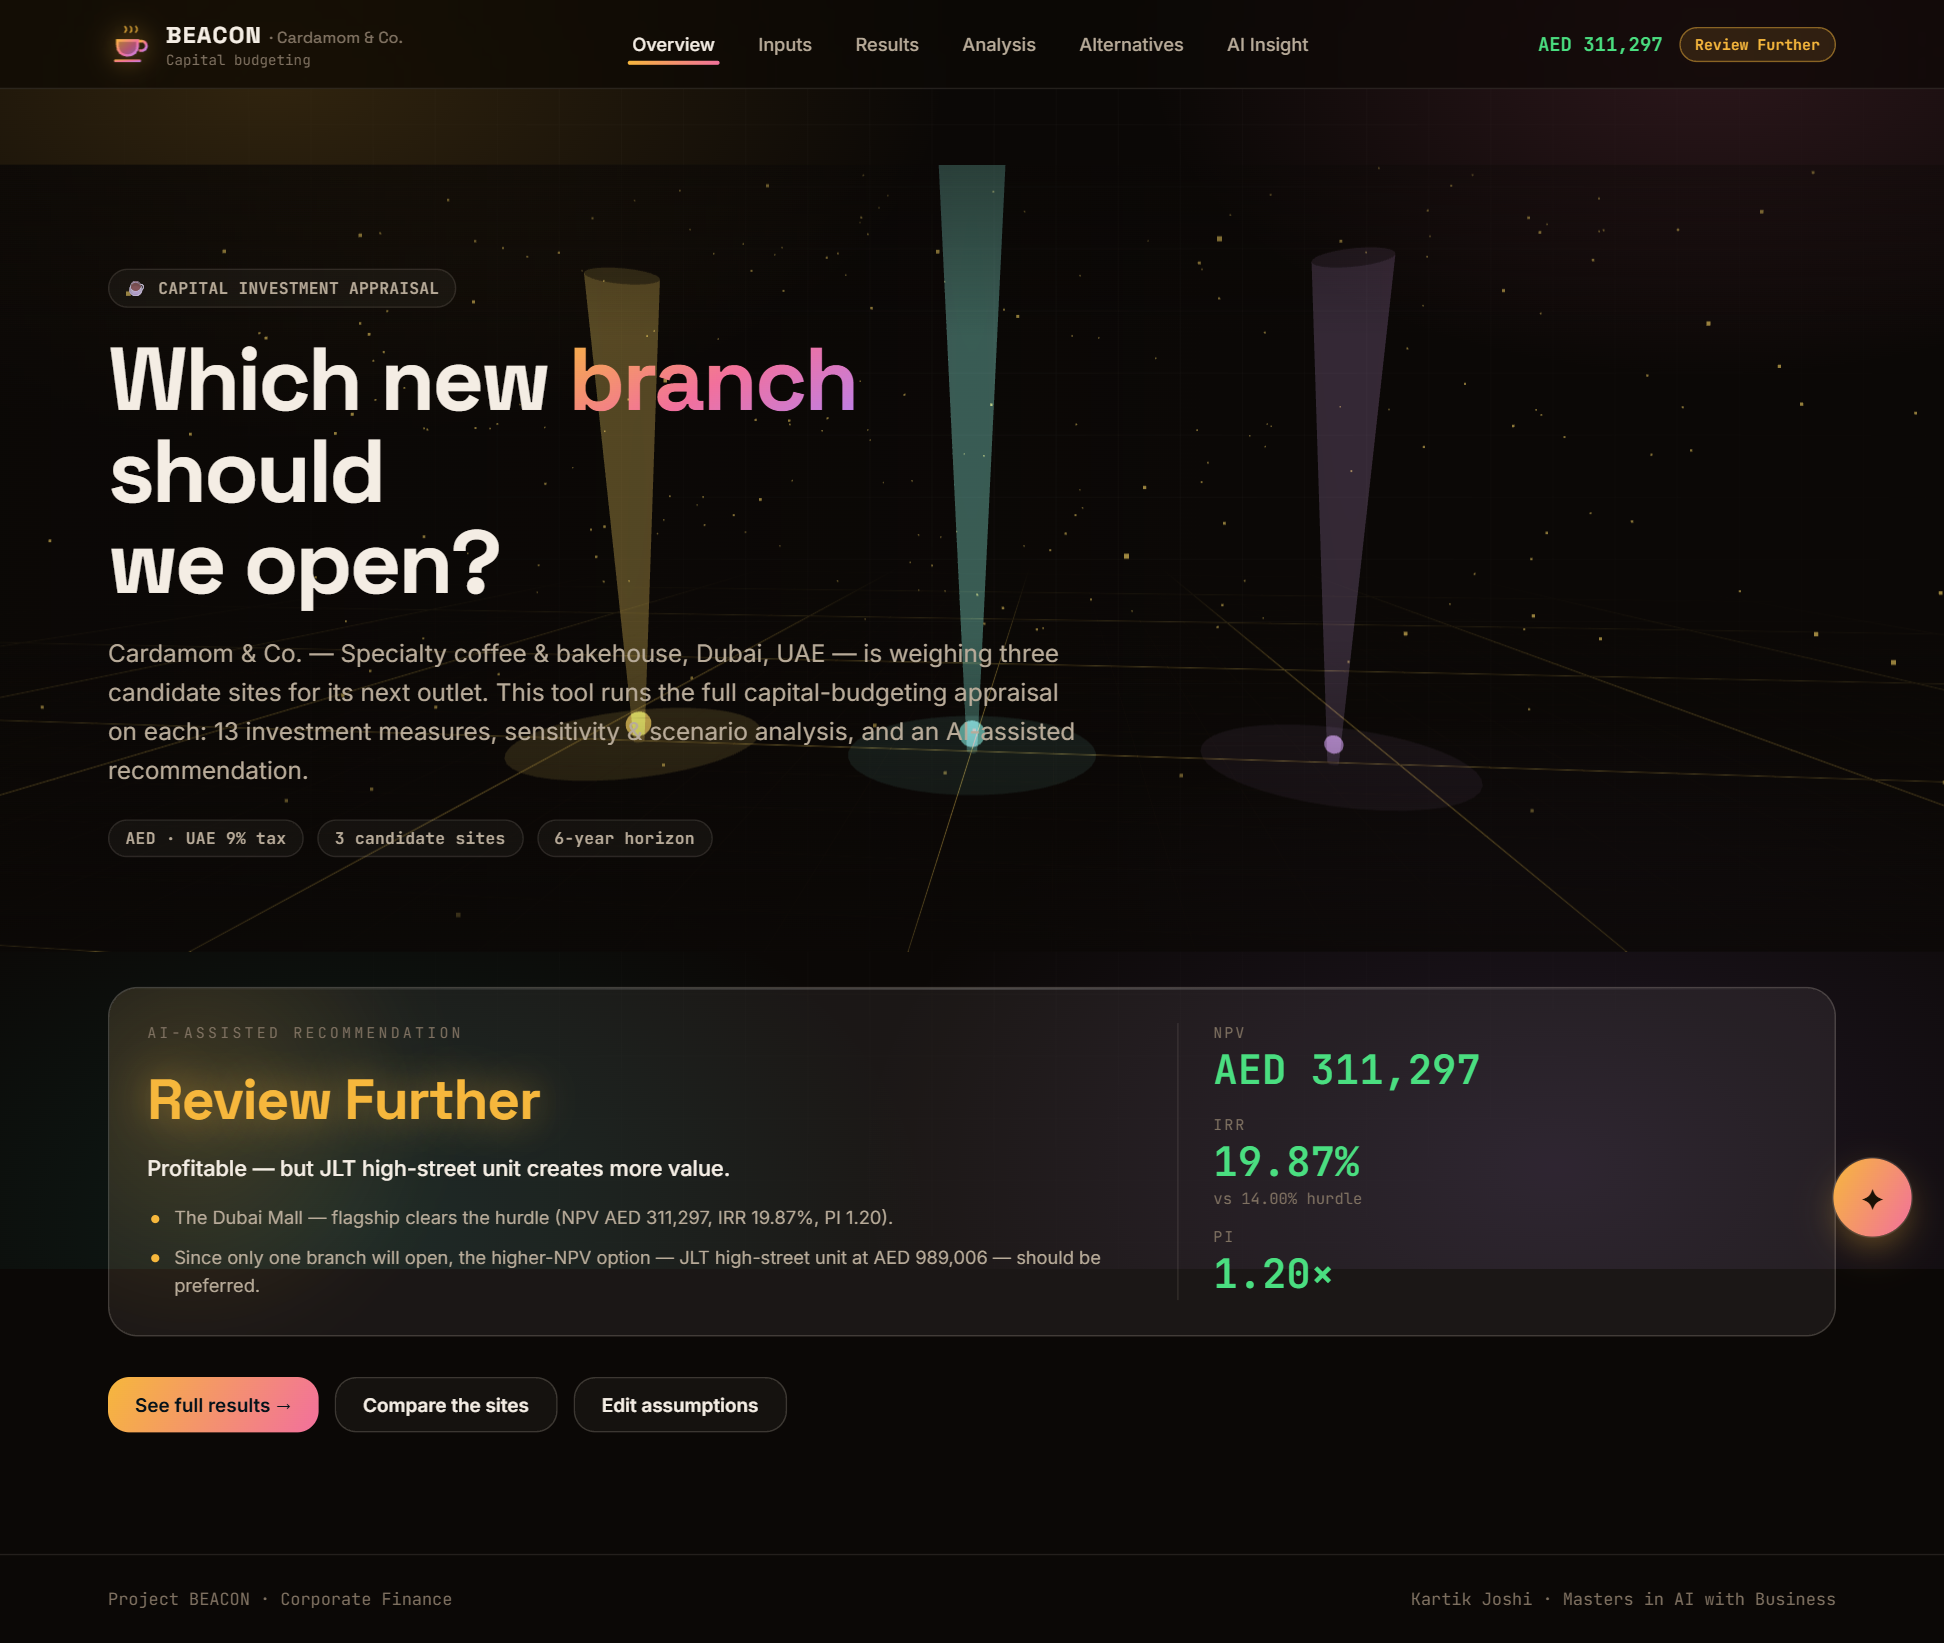
\includegraphics[width=0.92\linewidth]{01-overview.png}
\caption{Project BEACON overview --- the headline verdict and key metrics for the flagship site.}
\label{fig:overview}
\end{figure}

\section{Description of the Investment Decision}
The decision is a classic expansion / new-facility investment: commit roughly \aed 1.5~million of fit-out and working capital today in exchange for six years of operating cash flows and a terminal recovery. The managerial question is twofold: (i) does any single site create value at the firm's 14\% required return, and (ii) which site maximises shareholder value given the sites are mutually exclusive. Site~A (the flagship) is treated as the base project because it is the most visible and tempting; the analysis then tests whether that temptation is financially justified.

\section{Project Assumptions and Data Sources}
All values are in UAE dirhams (\aed). Estimates are benchmarked against typical Dubai food-and-beverage economics: mall rents and fit-out costs from commercial-leasing norms, coffee gross margins ($\approx 60\%$) from industry reports, and the 9\% UAE federal corporate-tax rate. The 14\% required return reflects an SME hurdle above the cost of debt. Revenue grows 6\% per year (same-store growth) and fixed costs escalate 3\% (rent and wage inflation). Depreciation is straight-line over the six-year lease. Site~A's assumptions are given in Table~\ref{tab:inputs}; the input form is shown in Figure~\ref{fig:inputs}.

\begin{table}[h]
\centering
\caption{Key inputs --- Site A (Dubai Mall flagship).}
\label{tab:inputs}
\begin{tabular}{@{}lr@{}}
\toprule
\textbf{Item} & \textbf{Value}\\
\midrule
Initial investment (fit-out \& equipment) & \aed 1{,}200{,}000\\
Installation \& transportation & \aed 180{,}000\\
Working capital (recovered at end) & \aed 150{,}000\\
Sunk cost (feasibility study --- \emph{excluded}) & \aed 40{,}000\\
Project life & 6 years\\
Year-1 revenue (growth 6\%/yr) & \aed 2{,}900{,}000\\
Fixed cost / yr (growth 3\%/yr) & \aed 1{,}550{,}000\\
Variable cost (\% of sales) & 36\%\\
Depreciation (straight-line) & \aed 200{,}000 / yr\\
Salvage value & \aed 180{,}000\\
Tax rate (UAE corporate) & 9\%\\
Required return (WACC) & 14\%\\
\bottomrule
\end{tabular}
\end{table}

\begin{figure}[h]
\centering
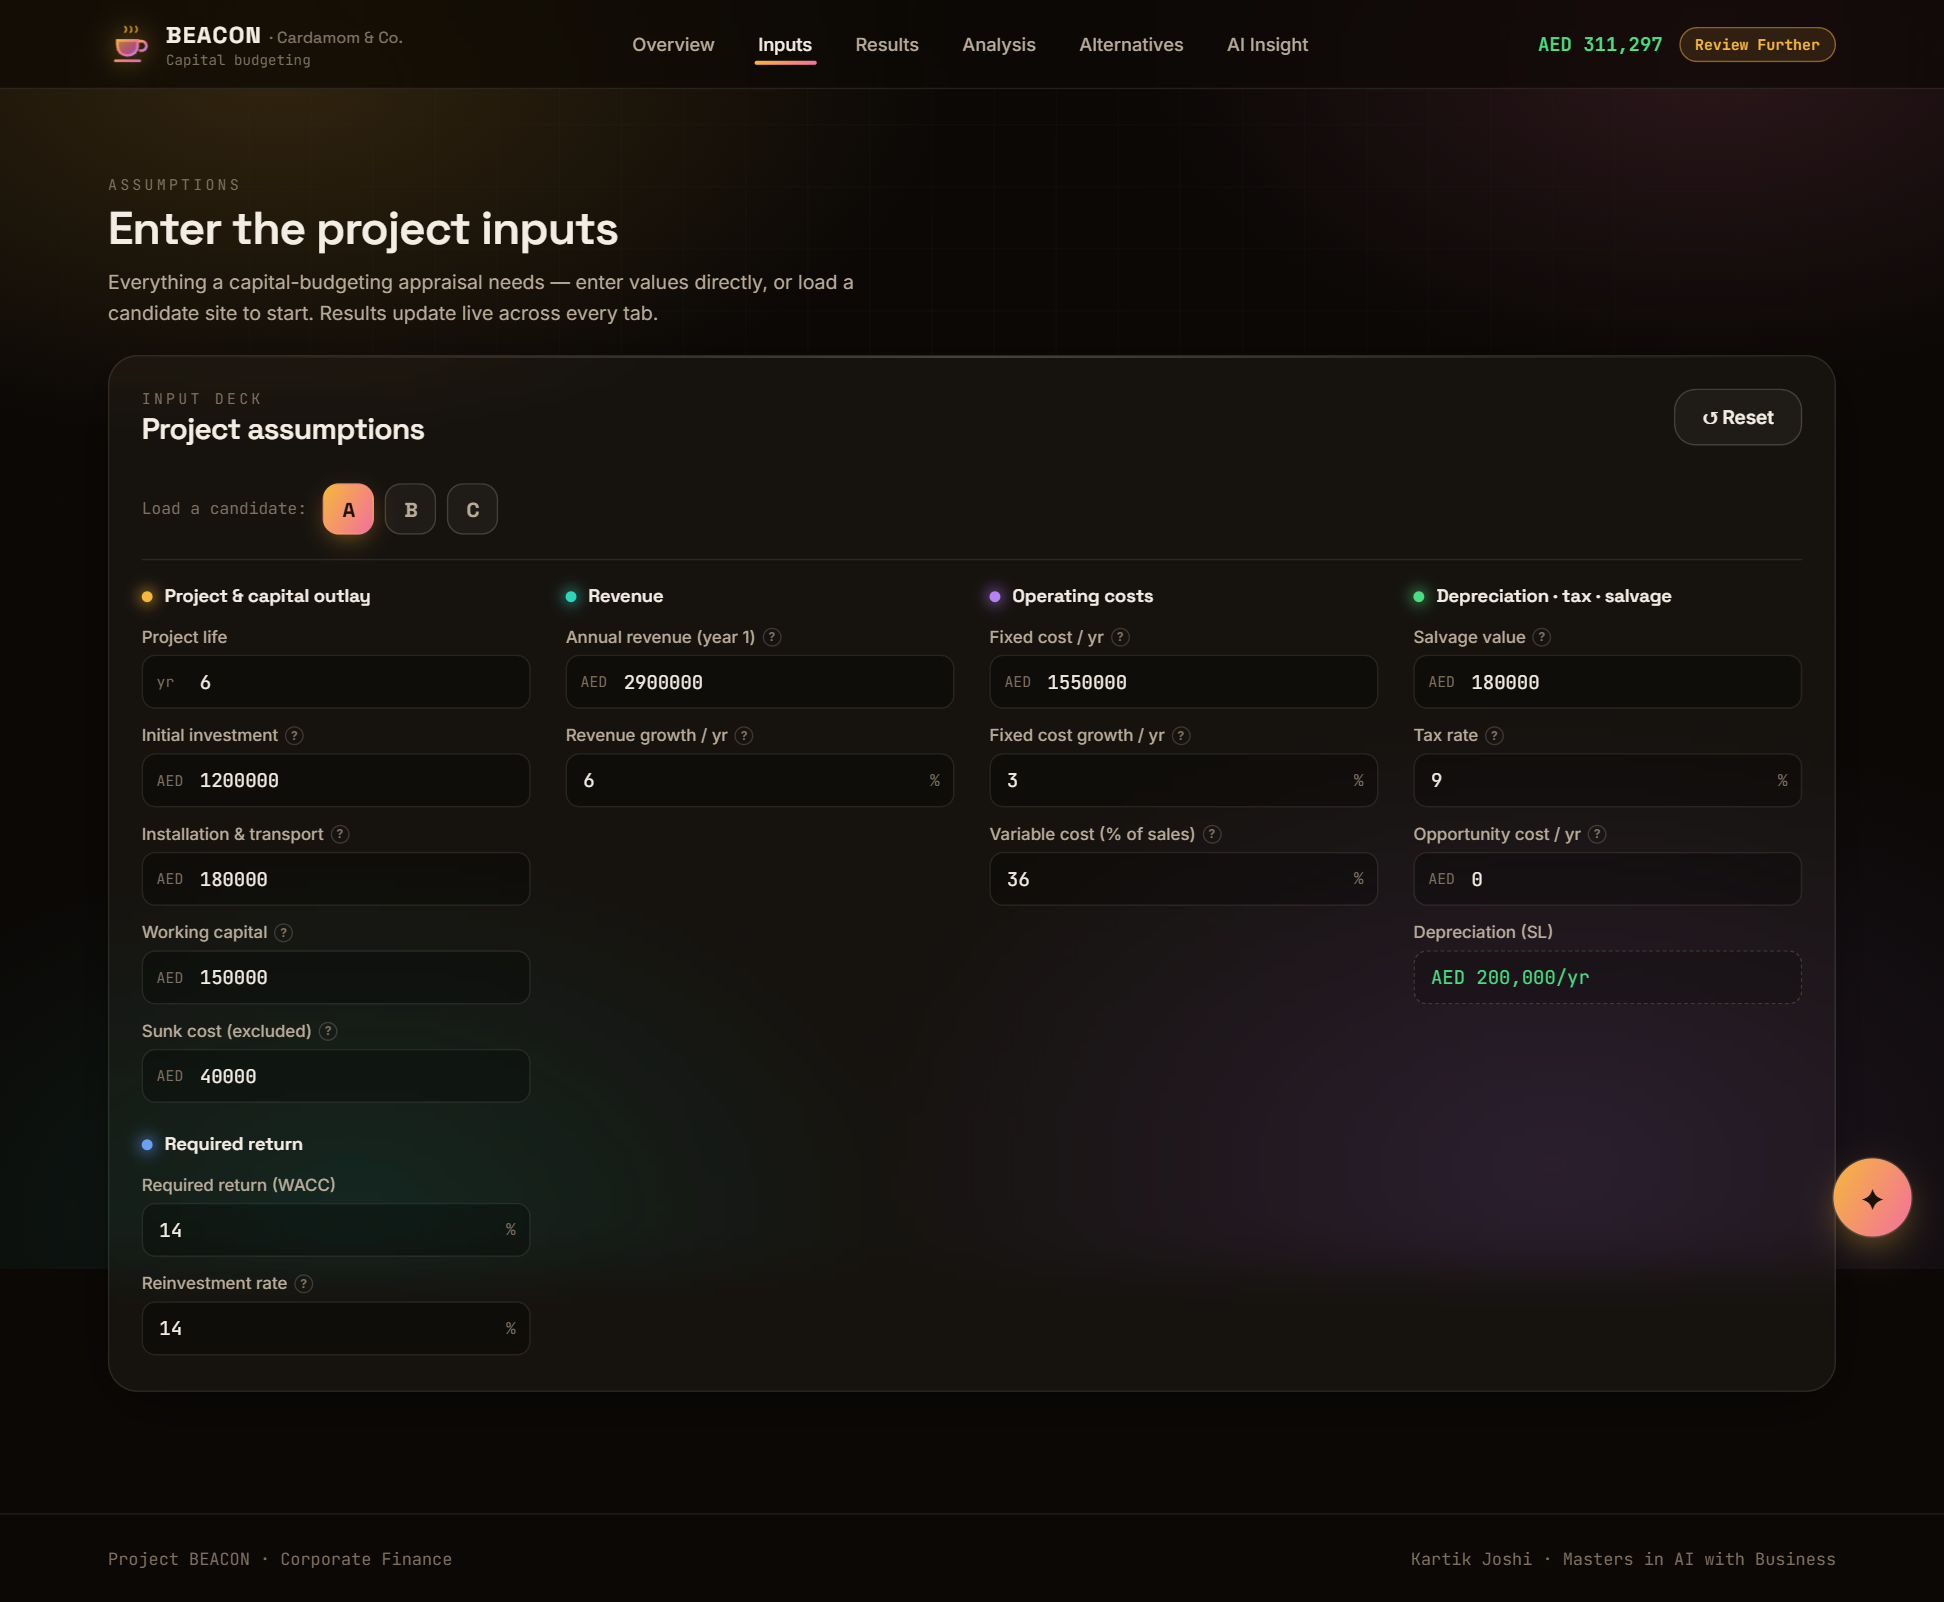
\includegraphics[width=0.92\linewidth]{02-inputs.png}
\caption{The generic, beginner-friendly input deck (all values shown for Site A).}
\label{fig:inputs}
\end{figure}

\section{Relevant and Irrelevant Cash Flows}
Only incremental, future cash flows attributable to the decision are included. \textbf{Relevant} flows are the fit-out and equipment outlay, installation and transportation, the working-capital investment and its recovery, the annual operating cash flows, and the after-tax salvage. The \aed 40{,}000 already spent on the feasibility and market study is a \textbf{sunk cost}: it is unaffected by the decision and is therefore \emph{excluded}, though the application deliberately displays it to make the exclusion explicit. Allocated head-office overhead that would exist regardless of the opening is likewise irrelevant and omitted.

\section{Treatment of Sunk Costs, Opportunity Costs, Working Capital, Depreciation, Taxes and Salvage}
\begin{itemize}[leftmargin=1.4em,itemsep=2pt]
\item \textbf{Sunk costs.} The \aed 40{,}000 study is excluded as irrelevant to the go/no-go decision.
\item \textbf{Opportunity costs.} The app accepts an annual opportunity-cost input (e.g.\ sub-letting the unit); it is set to zero here, while the capital's alternative use is captured through the 14\% discount rate.
\item \textbf{Working capital.} \aed 150{,}000 is invested at $t_0$ (inventory, supplier deposits, cash float) and fully recovered in the terminal year; it is not depreciated.
\item \textbf{Depreciation.} Straight-line, \aed 200{,}000/yr on the \aed 1{,}380{,}000 depreciable base (equipment~+~installation). It is non-cash but shields tax.
\item \textbf{Taxes.} 9\% UAE corporate tax on operating profit; early-year losses are assumed to offset group profits (symmetric treatment).
\item \textbf{Salvage.} The \aed 180{,}000 residual equals ending book value, so no disposal gain/loss arises; the engine applies disposal tax whenever salvage $\neq$ book value.
\end{itemize}

\section{Capital-Budgeting Calculations and Results}
Annual operating cash flow and the core measures are computed as:
\[
\text{OCF}_t = (\text{Rev}_t - \text{VC}_t - \text{FC}_t - D_t)(1-T) + D_t,
\qquad
\text{CF}_0 = -(\text{Equip}+\text{Install}+\text{WC}) = -\aed 1{,}530{,}000 .
\]
\[
\text{NPV}=\sum_{t=0}^{n}\frac{\text{CF}_t}{(1+r)^t},
\qquad
\text{PI}=\frac{\sum_{t=1}^{n}\text{CF}_t/(1+r)^t}{|\text{CF}_0|}=1+\frac{\text{NPV}}{|\text{CF}_0|},
\qquad
\text{IRR}:\ \sum_{t=0}^{n}\frac{\text{CF}_t}{(1+\text{IRR})^t}=0 .
\]
\[
\text{MIRR}=\left(\frac{\text{FV}_{\text{inflows}}^{\,r_{\text{re}}}}{-\,\text{PV}_{\text{outflows}}^{\,r_{\text{fin}}}}\right)^{1/n}\!-1,
\qquad
\text{ARR}=\frac{\overline{\text{Profit after tax}}}{\text{Average investment}},
\qquad
\text{BE revenue}=\frac{\text{FC}+D}{1-v},
\]
where $v$ is the variable cost as a fraction of sales. The six operating cash flows for Site~A are \aed 296{,}460, 355{,}483, 419{,}316, 488{,}287, 562{,}743 and 643{,}053, with a \aed 330{,}000 terminal recovery added in year~6. Results are summarised in Table~\ref{tab:results} and Figure~\ref{fig:results}; all figures were independently verified by a test harness (19/19 checks). On its own merits Site~A is value-creating, but its accounting break-even of \aed 2{,}734{,}375 --- a slim 94.3\% of first-year sales --- signals a thin margin of safety.

\begin{table}[h]
\centering
\caption{The thirteen required measures --- Site A.}
\label{tab:results}
\begin{tabular}{@{}lr@{}}
\toprule
\textbf{Measure} & \textbf{Result}\\
\midrule
Initial cash flow & \aed (1{,}530{,}000)\\
Terminal-year cash flow & \aed 330{,}000\\
Payback period & 3.94 years\\
Discounted payback period & 5.30 years\\
Accounting rate of return (ARR) & 33.45\%\\
Net present value (NPV) & \aed 311{,}297\\
Internal rate of return (IRR) & 19.87\%\\
Modified IRR (MIRR) & 17.57\%\\
Profitability index (PI) & 1.20\\
Break-even revenue (year 1) & \aed 2{,}734{,}375 (94.3\% of sales)\\
\bottomrule
\end{tabular}
\end{table}

\begin{figure}[h]
\centering
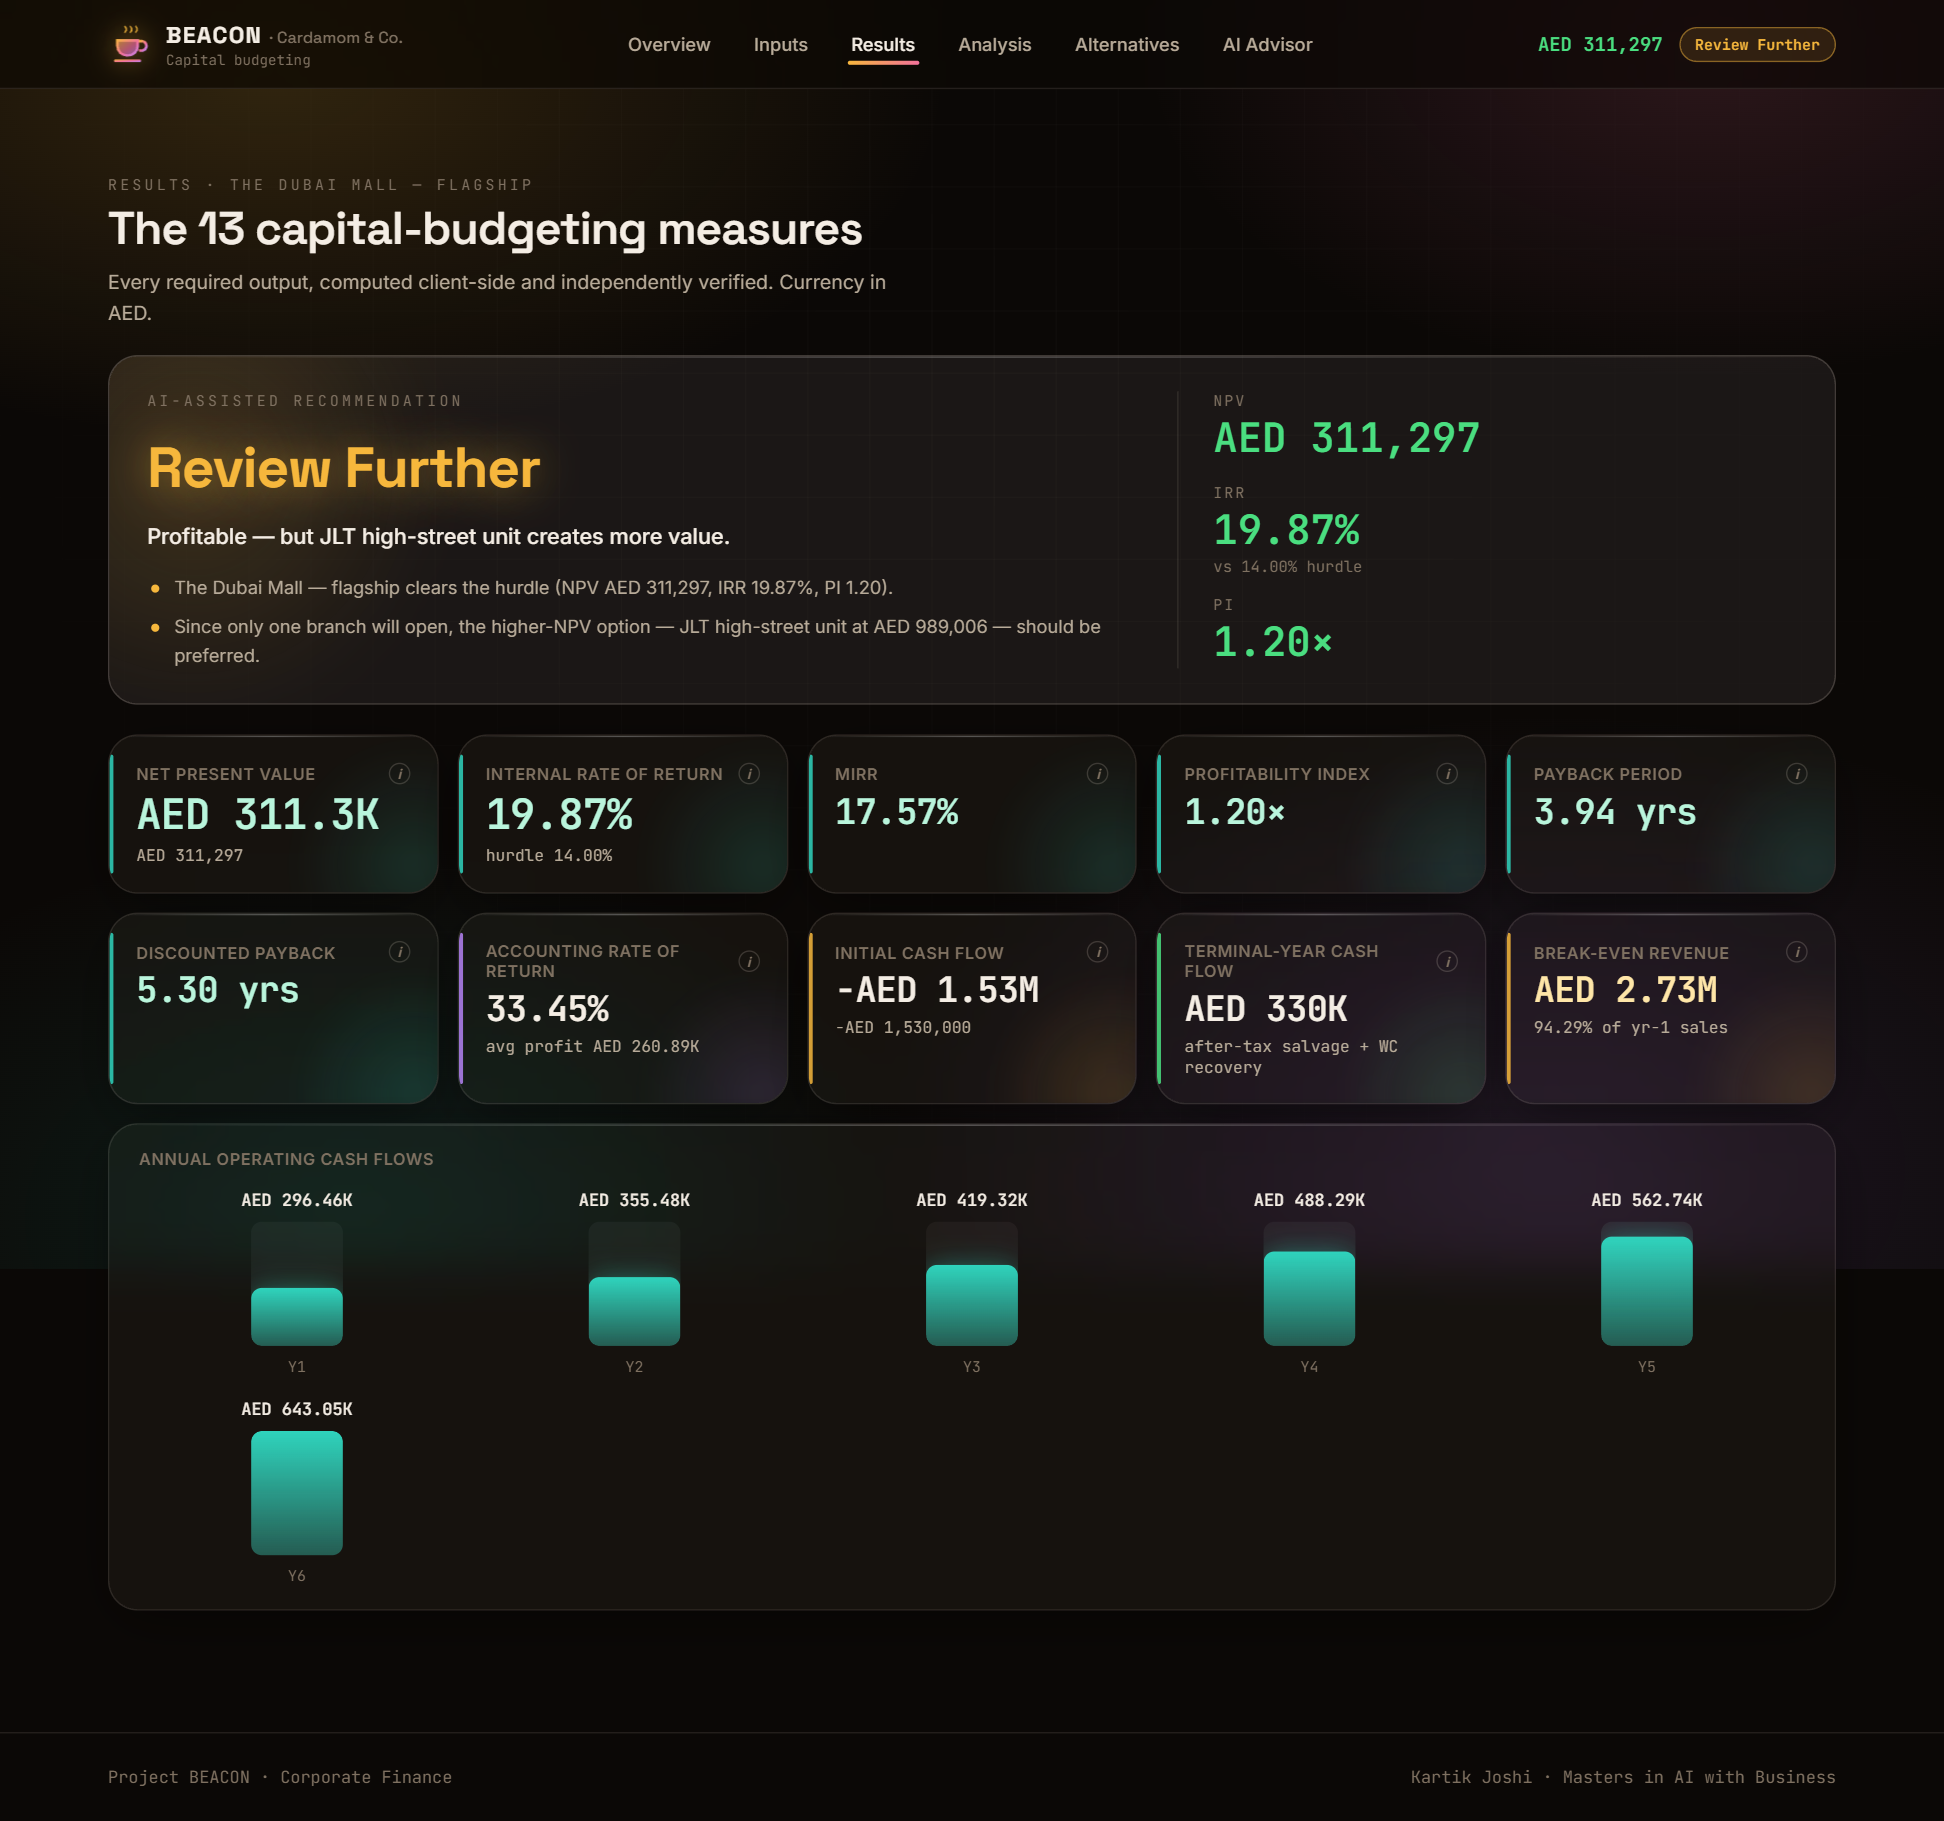
\includegraphics[width=0.92\linewidth]{03-results.png}
\caption{Results dashboard --- the 13 capital-budgeting measures for Site A.}
\label{fig:results}
\end{figure}

\section{Comparison of Investment Alternatives}
Because the sites are mutually exclusive, the correct selection criterion is the \textbf{highest NPV}, not the highest IRR or PI (which can favour smaller-scale projects). Table~\ref{tab:alts} and Figure~\ref{fig:alts} rank them. Site~B (JLT) dominates with an NPV of \aed 989{,}006 --- more than triple Site~A --- because its far lower rent preserves margin despite lower revenue. Site~C (cloud kitchen) is capital-light and posts the second-highest NPV. The glamorous flagship (Site~A) is, paradoxically, the weakest: premium mall rent erodes its thin contribution.

\begin{table}[h]
\centering
\caption{Alternatives ranked by NPV (mutually exclusive --- only one opens).}
\label{tab:alts}
\begin{tabular}{@{}lrrrr@{}}
\toprule
\textbf{Site} & \textbf{NPV} & \textbf{IRR} & \textbf{PI} & \textbf{Payback}\\
\midrule
B --- JLT high-street & \aed 989{,}006 & 40.9\% & 1.99 & 2.42 yr\\
C --- Delivery cloud kitchen & \aed 325{,}328 & 32.9\% & 1.69 & 2.92 yr\\
A --- Dubai Mall flagship & \aed 311{,}297 & 19.9\% & 1.20 & 3.94 yr\\
\bottomrule
\end{tabular}
\end{table}

\begin{figure}[h]
\centering
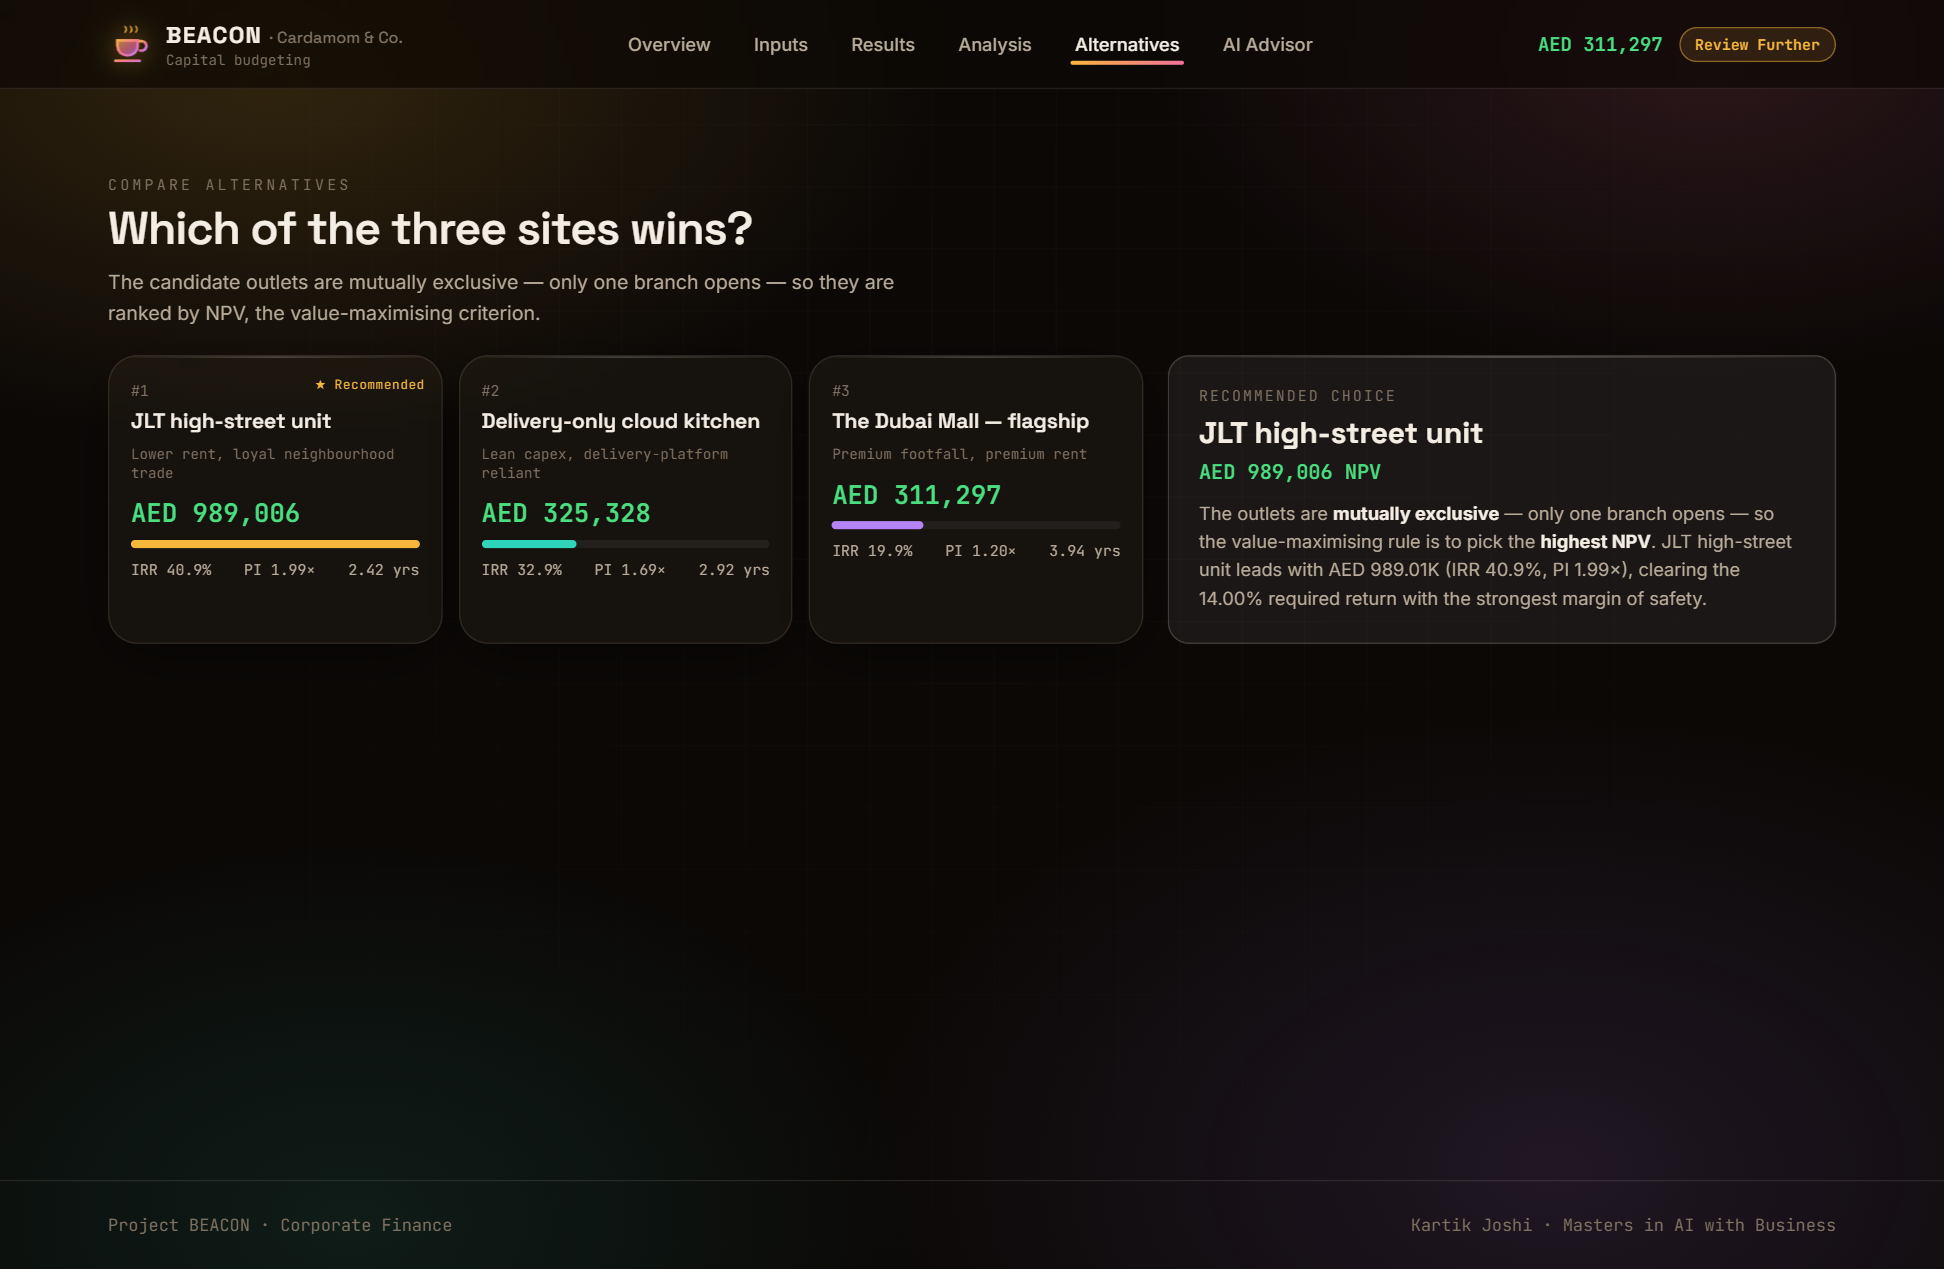
\includegraphics[width=0.92\linewidth]{05-alternatives.png}
\caption{Alternatives comparison --- Site B is the value-maximising choice.}
\label{fig:alts}
\end{figure}

\section{Sensitivity and Scenario Analysis}
A one-at-a-time sensitivity on Site~A ($\pm 20\%$, Figure~\ref{fig:analysis}) shows NPV is most exposed to \textbf{sales revenue} (swing $\approx$ \aed 3.0m) and \textbf{fixed rent} ($\approx$ \aed 2.2m); a 20\% revenue shortfall alone turns NPV sharply negative. Combined best/base/worst scenarios span \aed $-1.36$m to $+2.17$m (Table~\ref{tab:scen}), and the decision \emph{flips} between them --- confirming the flagship's fragility and the value of choosing the lower-rent Site~B instead.

\begin{table}[h]
\centering
\caption{Scenario analysis --- Site A.}
\label{tab:scen}
\begin{tabular}{@{}lrrr@{}}
\toprule
\textbf{Scenario} & \textbf{NPV} & \textbf{IRR} & \textbf{PI}\\
\midrule
Worst & \aed (1{,}355{,}530) & $-11.4\%$ & 0.18\\
Base & \aed 311{,}297 & 19.9\% & 1.20\\
Best & \aed 2{,}167{,}200 & 51.0\% & 2.47\\
\bottomrule
\end{tabular}
\end{table}

\begin{figure}[h]
\centering
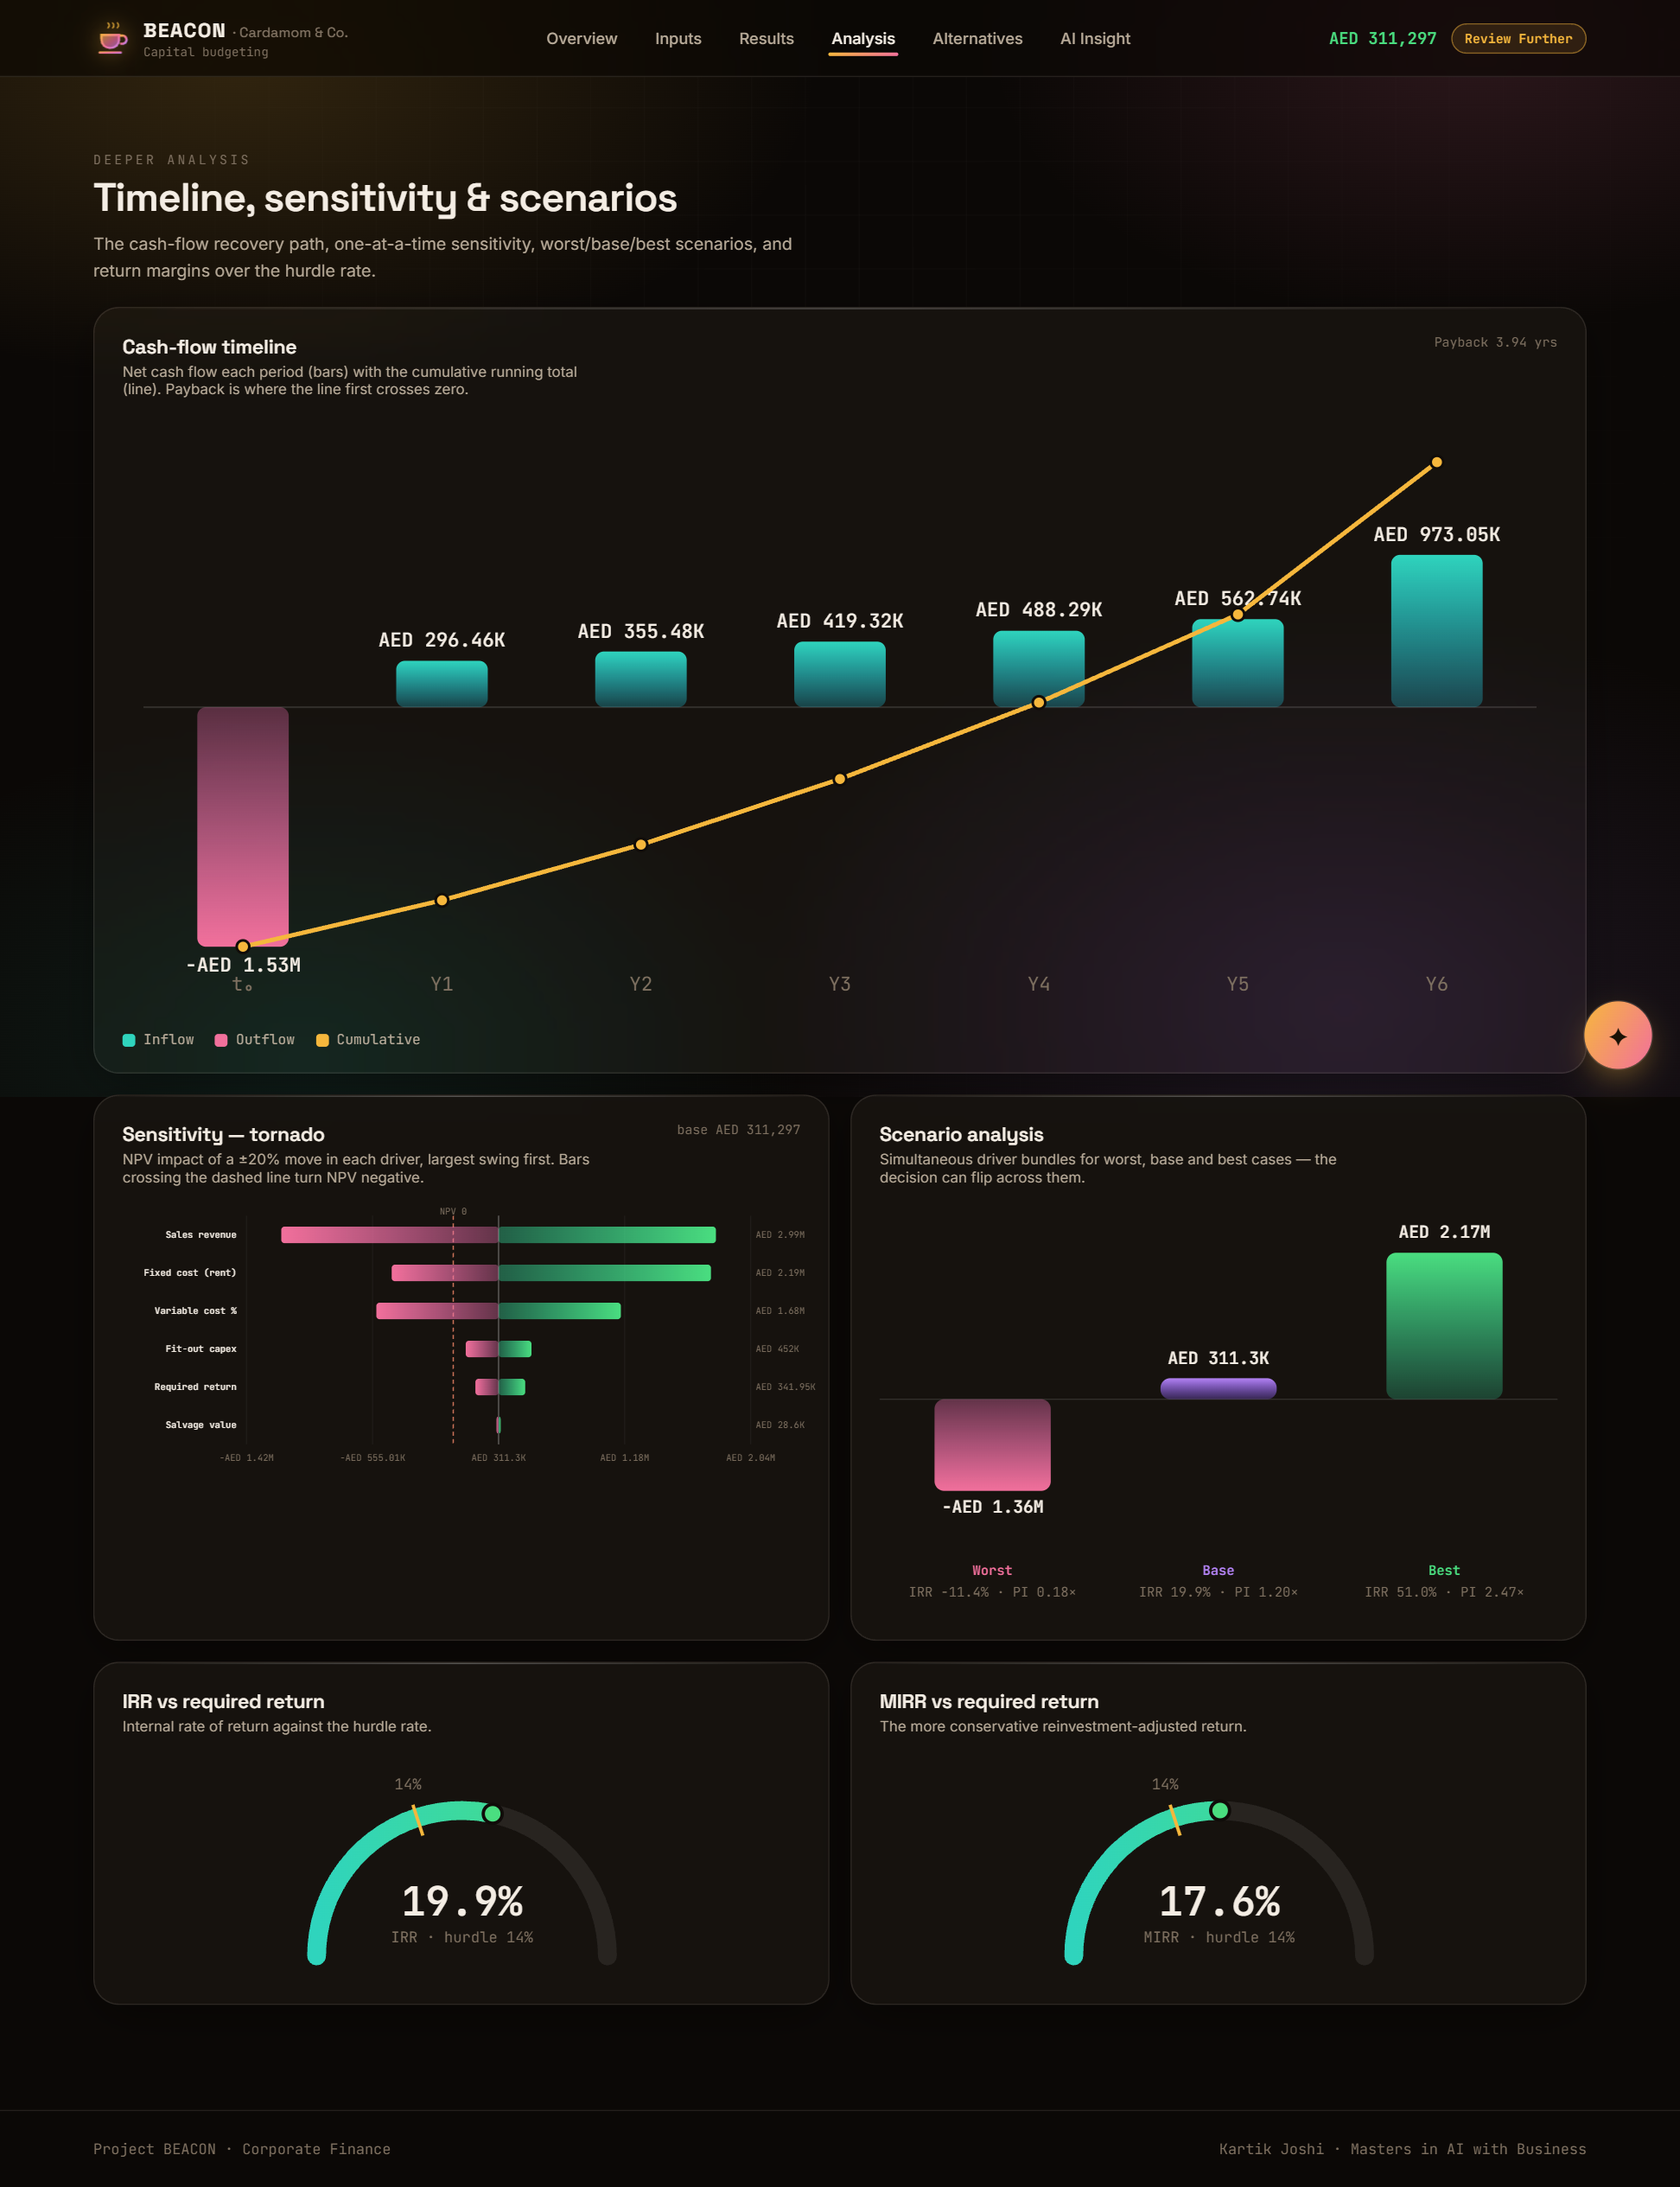
\includegraphics[width=0.92\linewidth]{04-analysis.png}
\caption{Cash-flow timeline, sensitivity tornado, scenarios and return gauges.}
\label{fig:analysis}
\end{figure}

\section{Financial and Non-Financial Risks}
\textbf{Financial:} high operating leverage (rent and payroll dominate the cost base); demand / footfall risk (the single largest NPV driver); input-cost inflation compressing the $\approx 60\%$ gross margin; and fit-out cost overruns that lengthen payback. \textbf{Non-financial:} dependence on a single high-traffic location and its lease-renewal terms; intense caf\'e-market saturation in Dubai; staffing and service-consistency risk; and --- for the cloud-kitchen option --- reliance on delivery-aggregator commissions that can be changed unilaterally.

\section{AI-Generated Insights and Student Evaluation}
The application's AI advisor (Figures~\ref{fig:aiinsight}--\ref{fig:aichat}), an NVIDIA-hosted large language model grounded in the computed metrics, recommended opening the JLT high-street unit, citing its highest NPV (\aed 989{,}006), IRR (40.9\%) and shortest payback (2.42 years). \textbf{Student evaluation:} the AI's reasoning is sound and coincides with my own analysis, which raises confidence in the conclusion. However, its judgement is only as good as the numbers it is given: it correctly applies the NPV rule for mutually-exclusive projects and flags the thin margin of safety, but it does not interrogate the \emph{quality} of the assumptions, stress-test them, or weigh non-financial factors such as the brand value of a mall flagship or the durability of JLT footfall. I therefore treat the AI as \emph{decision-support} --- valuable for fast, plain-language synthesis and sanity-checking --- rather than a substitute for the analyst's judgement.

\begin{figure}[h]
\centering
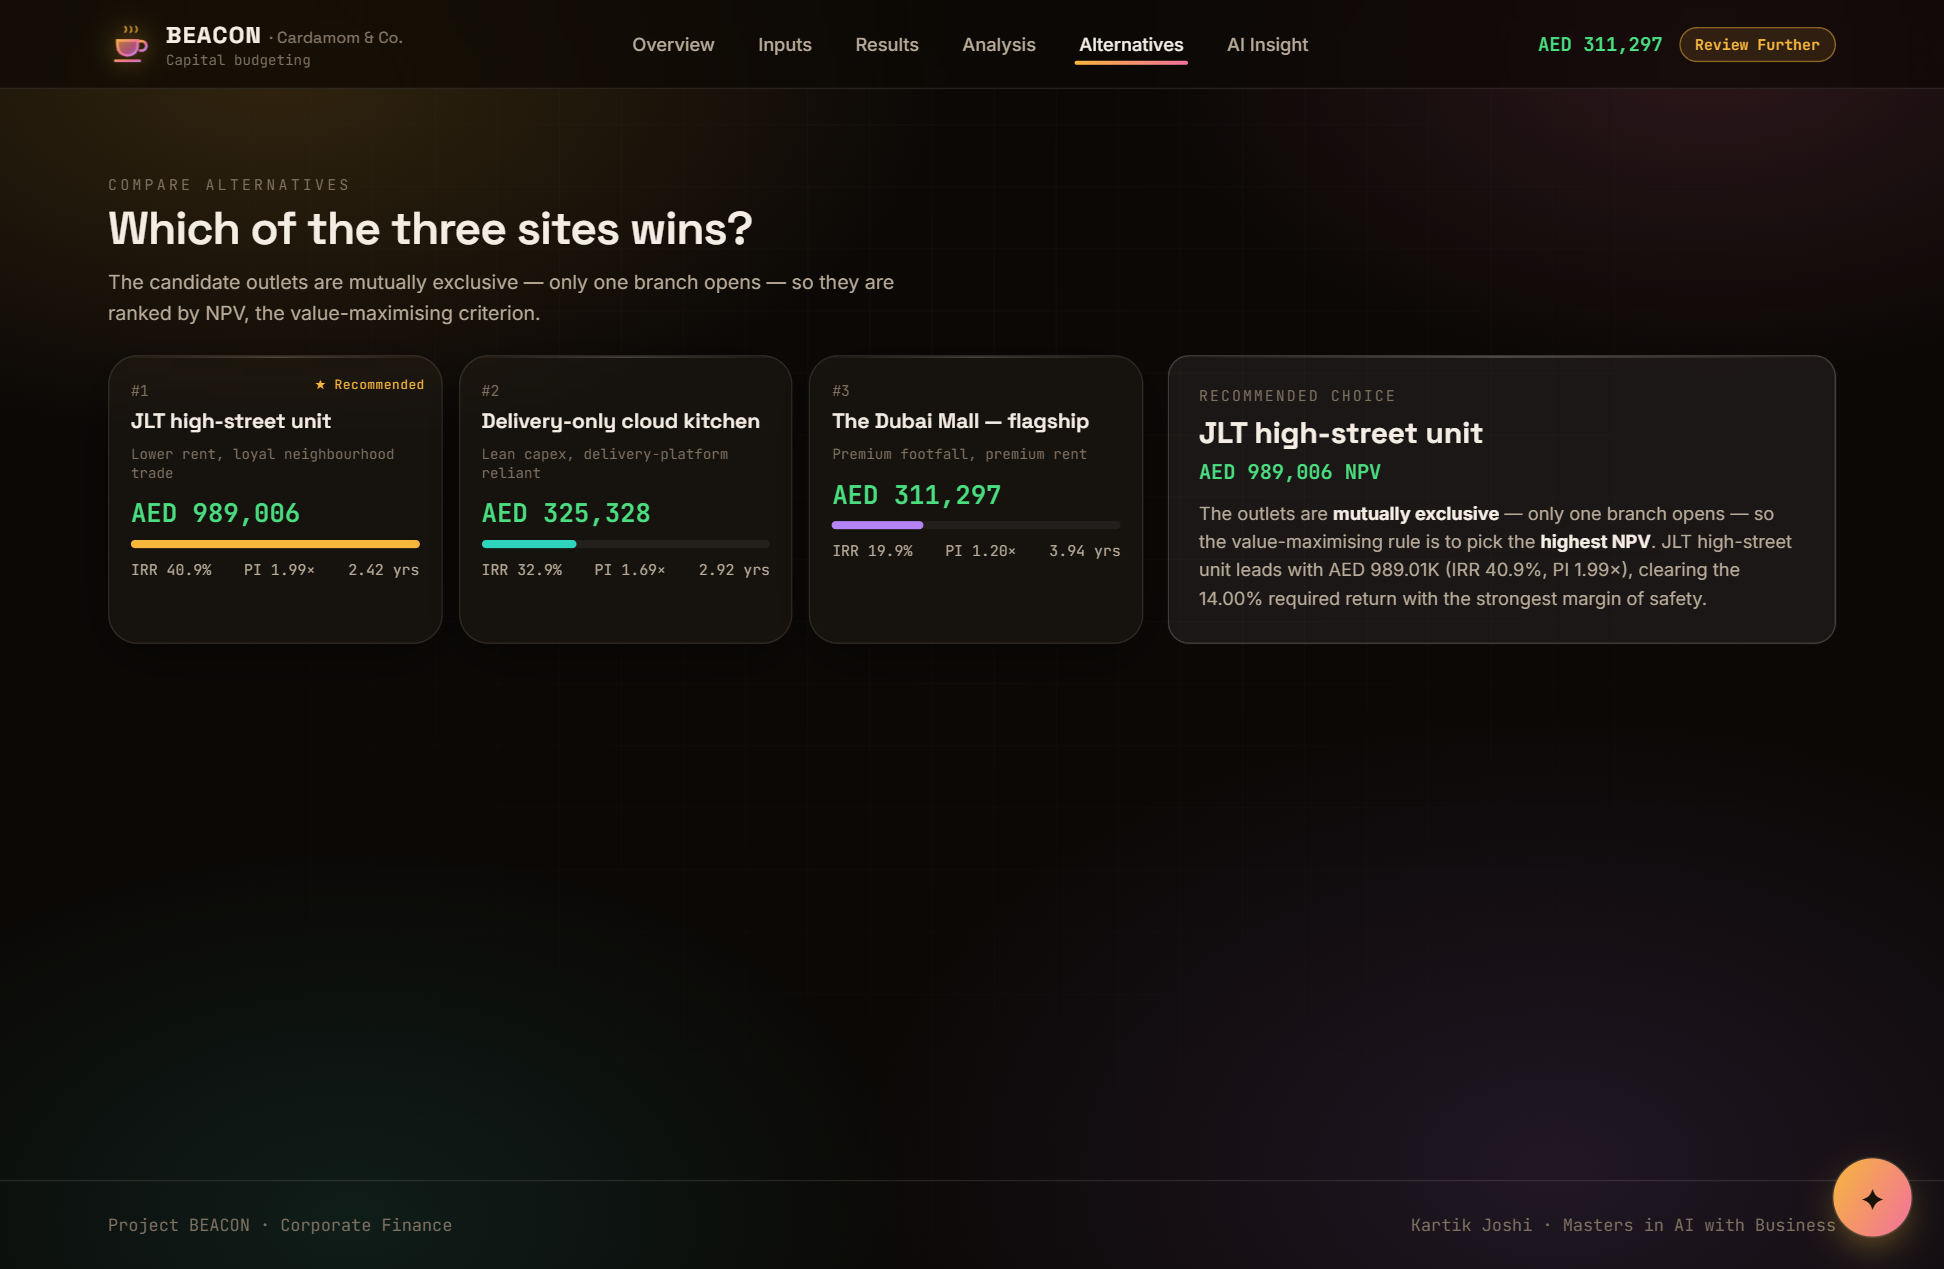
\includegraphics[width=0.92\linewidth]{06-ai-insight.png}
\caption{AI Insight --- plain-language explanation, risk register and recommendation.}
\label{fig:aiinsight}
\end{figure}

\begin{figure}[h]
\centering
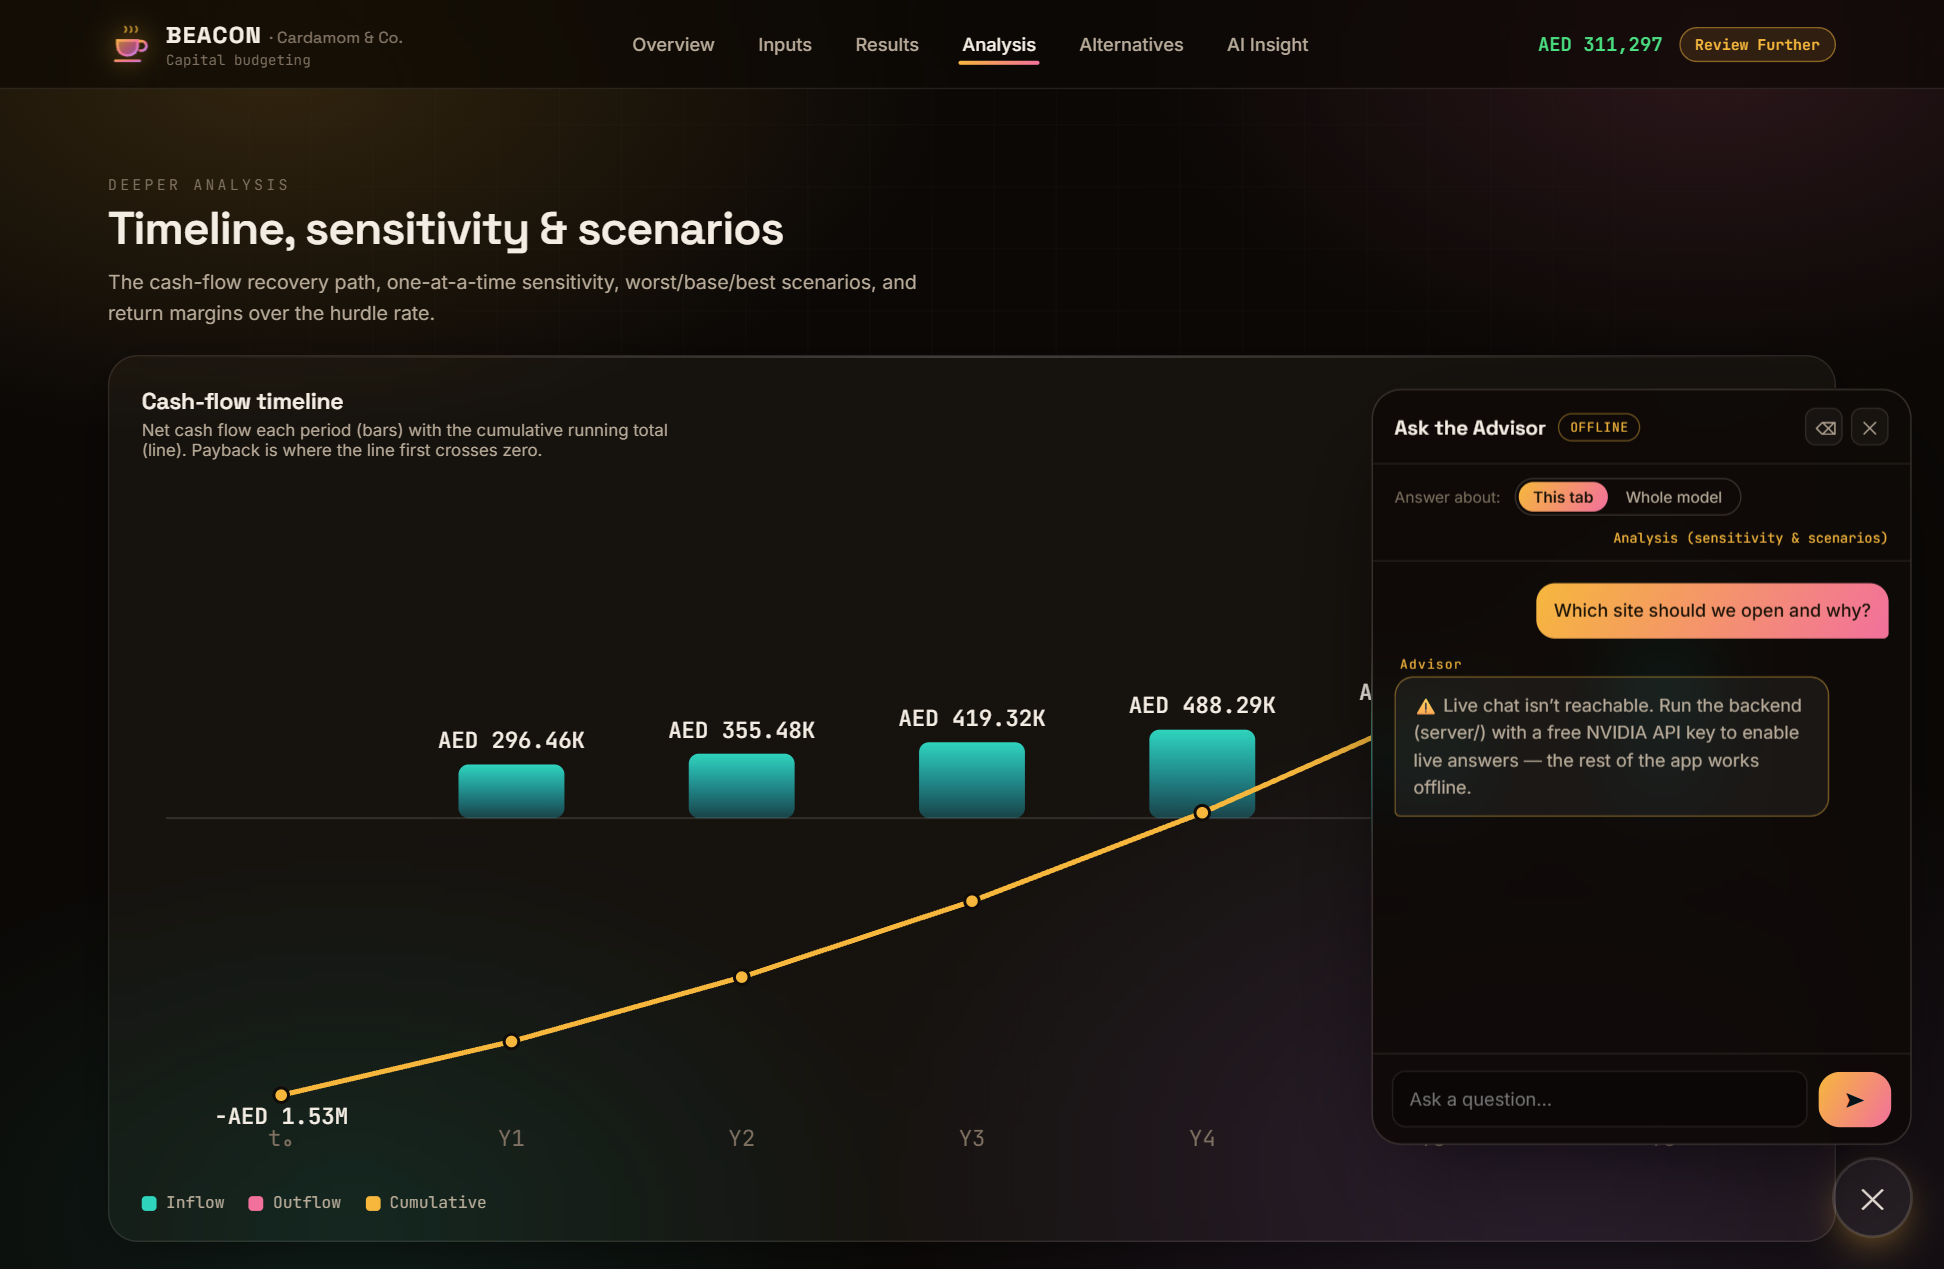
\includegraphics[width=0.6\linewidth]{07-ai-chat.png}
\caption{The floating, tab-aware ``Ask the Advisor'' chat answering live from the metrics.}
\label{fig:aichat}
\end{figure}

\section{Final Investment Recommendation}
\textbf{Recommendation: open Site~B, the JLT high-street unit --- Accept.} It maximises shareholder value (NPV \aed 989{,}006), comfortably clears the 14\% hurdle (IRR 40.9\%) and recovers capital fastest (2.42 years). The flagship (Site~A) should be \emph{rejected} in this round: although positive-NPV in isolation, it is dominated by Site~B and is dangerously sensitive to a revenue shortfall. Site~C is a viable capital-light fallback should the JLT lease fall through.

\section{Limitations of the Analysis}
The appraisal rests on management's point estimates; revenue and rent --- the dominant drivers --- are uncertain and could materially change the outcome. Cash flows are projected over a fixed six-year horizon with a single tax and discount rate, ignoring financing structure and possible mid-life refurbishment. The scenarios are illustrative bundles rather than a full Monte-Carlo distribution, and qualitative strategic value (the brand visibility of a mall flagship) is not monetised.

% ======================================================================
% REFERENCES & DECLARATION
% ======================================================================
\section*{References}
\addcontentsline{toc}{section}{References}
\begin{enumerate}[leftmargin=1.6em,itemsep=1pt]
\item Ross, S., Westerfield, R.\ \& Jaffe, J. \emph{Corporate Finance}. McGraw-Hill.
\item Brealey, R., Myers, S.\ \& Allen, F. \emph{Principles of Corporate Finance}. McGraw-Hill.
\item UAE Federal Tax Authority --- Corporate Tax (9\%). \href{https://tax.gov.ae}{tax.gov.ae}.
\item NVIDIA API documentation. \href{https://build.nvidia.com}{build.nvidia.com}.
\item Application source code and live deployment: \href{https://github.com/KartikJoshi23/Beacon}{github.com/KartikJoshi23/Beacon} \textbullet\ \href{https://beacon-intelligence.vercel.app/}{beacon-intelligence.vercel.app}.
\end{enumerate}

\section*{Declaration of AI Tools Used}
\addcontentsline{toc}{section}{Declaration of AI Tools Used}
The application and this report were developed with \textbf{Claude Code} (Anthropic) as the engineering assistant. The application's runtime AI advisor uses an \textbf{NVIDIA-hosted Llama-3.1-8B-Instruct} model via the NVIDIA API, with a deterministic offline fallback for reliability. All financial formulas were implemented and \emph{independently verified} by the author (19/19 automated checks); AI outputs were critically reviewed and were not accepted uncritically. The final judgement and recommendation are the author's own.

\vfill
\begin{center}\small\itshape Kartik Joshi --- Masters in Artificial Intelligence with Business.\end{center}

\end{document}
